\documentclass{seminar}
\usepackage{color}
\usepackage[colorlinks,urlcolor=blue,linkcolor=black,citecolor=black]{hyperref}
\usepackage{gensymb}
\usepackage{amsmath,amssymb}
\usepackage{bm}
\usepackage{graphicx}
\usepackage{parskip}
%\parindent=0pt
\setcounter{tocdepth}{1}
%-----------------------------------------------------------
\title{PHY478F Undergraduate Research Project\\on\\Hydrodynamic Stability}
\author{Man-Wai Yau\thanks{Supervisor: Prof.~W.R.~Peltier}}
\date{December 20, 2006}
%-----------------------------------------------------------
\begin{document}
\begin{slide}
\maketitle
\newslide
%-----------------------------------------------------------
\begin{abstract}
This undergraduate research project focused upon the problem of
hydrodynamic stability, specifically on the aspect of this general
class of problems that involves the transition to turbulence in
density stratified shear flows. The conservation laws of mass and
momentum were studied. The equation of motion, Navier-Stokes
equation, was derived from the conservation laws. Reyleigh's
stability equation and Taylor-Goldstein equation were used to
investigate the mechanisms of transition of the Kelvin-Helmholtz and
Holmboe modes of instability.
\end{abstract}
\newslide
%-----------------------------------------------------------
\tableofcontents
%-----------------------------------------------------------
\newslide
\section{Background}
\subsection{Material Derivative}
\begin{align}
    \frac{Df}{Dt} &= \frac{\partial f}{\partial t}+\frac{\partial f}{\partial x}
    \frac{\partial x}{\partial t}+\frac{\partial f}{\partial
    y}\frac{\partial y}{\partial t}+\frac{\partial f}{\partial
    z}\frac{\partial z}{\partial t}\notag\\
    &= \frac{\partial f}{\partial
    t}+(\mathbf{u}\cdot\nabla)f
\end{align}
where $\mathbf{u}$ is the velocity of the packet.

\newslide
\section{Conservation Laws}
\subsection{Conservation of Mass}
Consider a small test volume $V$
with surface $A$. The rate of change of the mass in the volume is
\begin{equation}\label{mass:rate}
    \frac{d}{dt}\int_V\rho\,dV =
    \int_V\frac{\partial\rho}{\partial t}\,dV
\end{equation}
The derivative can be moved inside the integral because the test
volume is fixed in position.

The mass flow out of the surface is given by
\begin{equation}
    \int_A\rho\mathbf{u}\cdot\mathbf{n}\,dA =
    \int_V\nabla\cdot(\rho\mathbf{u})\,dV
\end{equation}
where divergence theorem was used to change the equation into a
volume integral.

From the law of conservation of mass, the rate of change of the mass
in the volume must be equal to the mass flow \emph{into} the
surface, thus
\begin{align}
    &\int_V\frac{\partial\rho}{\partial t}\,dV =
    -\int_V\nabla\cdot(\rho\mathbf{u})\,dV\notag\\
    &\int_V\Bigl[(\frac{\partial\rho}{\partial t}+\nabla\cdot(\rho\mathbf{u})\Bigr]\,dV = 0\label{mass:con}
\end{align}
Since the test volume is arbitrary, the function inside the bracket
[ ] must vanish everywhere. Hence
\begin{equation}\label{mass:cont}
\boxed{\frac{\partial\rho}{\partial t}+\nabla\cdot(\rho\mathbf{u}) =
0}
\end{equation}
\eqref{mass:cont} is called the equation of continuity. It can be
written in material derivative:
\begin{equation}\label{mass:cont2}
\frac{D\rho}{Dt}+\rho\nabla\cdot\mathbf{u} = 0
\end{equation}
For an incompressible fluid, $D\rho/Dt=0$, the equation of
continuity is reduced to
\begin{equation}\label{mass:cont3}
\nabla\cdot\mathbf{u} = 0
\end{equation}
\subsection{Conservation of Momentum} From the law of conservation of
momentum, consider a same fixed volume $V$:
\begin{equation}\label{mom:con}
    \frac{d}{dt}(\text{momentum in }V)= - \text{momentum leakage} +
    \sum(\text{applied force})
\end{equation}
The rate of change of mometum in the volume is
\begin{equation}\label{mom:rate}
    \frac{d}{dt}\int_V\rho u_i\,dV =
    \int_V\frac{\partial\rho u_i}{\partial t}\,dV
\end{equation}
where $u_i$ is the $i$th component of the velocity $\mathbf{u}$.
Similar to \eqref{mass:rate}, the derivative can be moved inside the
integral.

The momentum leakage (in component form) is given by
\begin{equation}\label{mom:leakage}
    \int_A(\rho u_i)u_j(n_j\,dAj) =
    \int_V\frac{\partial}{\partial x_j}(\rho u_i u_j)\,dV
\end{equation}
where divergence theorem was applied again.

The applied forces consist of body force and surface force. The body
force is simply
\begin{equation}\label{mom:bodyf}
    \text{body force} = \int_V\rho f_i\,dV
\end{equation}
where $f_i$ is the component of the body force per unit mass.

To find the surface force, I considered a tetrahedral volume of
fluid. The sum of the surface force must be zero by Newton's second
law\footnote{Otherwise it will be accelerating.}. The area of the
``big triangle'' is given by $\delta A$, while the area of other
three surfaces are given by
\begin{subequations}
\begin{align}
    \delta A_1&=\mathbf{a}\cdot \mathbf{n} \delta A\\
    \delta A_2&=\mathbf{b}\cdot \mathbf{n} \delta A\\
    \delta A_3&=\mathbf{c}\cdot \mathbf{n} \delta A
\end{align}
\end{subequations}
\begin{figure}[htpb]
  \centering
  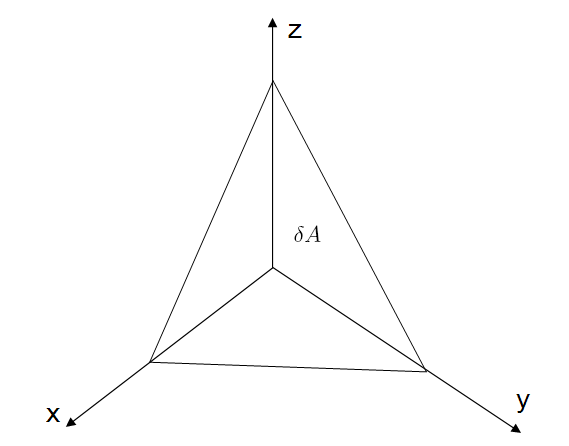
\includegraphics[width=0.7\textwidth]{stress.png}\\
  \caption{Stress on a tetrahedral volume of fluid}\label{stress}
\end{figure}

The sum of surface force is
\begin{align}
    \Sigma_i(\mathbf{n})\delta A + \Sigma_i(-\mathbf{a})\delta A_1 + \Sigma_i(-\mathbf{b})\delta
    A_2 + \Sigma_i(-\mathbf{c})\delta A_3 = 0\notag\\
    \Sigma_i(\mathbf{n})\delta A - \Sigma_i(\mathbf{a})\mathbf{a}\cdot \mathbf{n}\delta A
     - \Sigma_i(\mathbf{b})\mathbf{b}\cdot \mathbf{n}\delta
    A - \Sigma_i(\mathbf{c})\mathbf{c}\cdot \mathbf{n}\delta A = 0
\end{align}
Since $\Sigma$ is an odd function by Newton's third law. Then
\begin{equation}\label{mom:surf1}
    \Sigma_i(\mathbf{n}) = [ a_j\Sigma_i(\mathbf{a}) + b_j\Sigma_i(\mathbf{b}) +
    c_j\Sigma_i(\mathbf{c})] n_j
\end{equation}
So I can define the stress vector as
\begin{equation}\label{mom:surf1}
    \sigma_{ij} = a_j\Sigma_i(\mathbf{a}) + b_j\Sigma_i(\mathbf{b}) +
    c_j\Sigma_i(\mathbf{c})
\end{equation}
The total force on a surface is
\begin{equation}\label{mom:surf}
    \text{surface force} = \int_A\sigma_{ij}n_j\,dA = \int_V\frac{\partial}{\partial x_j}\sigma_{ij}\,dV
\end{equation}
Combining \eqref{mom:rate}, \eqref{mom:leakage}, \eqref{mom:bodyf}
and \eqref{mom:surf}, \eqref{mom:con} can be written as:
\begin{equation}\label{mom:con2}
    \int_V\frac{\partial\rho u_i}{\partial t}\,dV = - \int_V\frac{\partial}{\partial x_j}(\rho u_i
    u_j)\,dV + \int_V\rho f_i\,dV + \int_V\frac{\partial}{\partial x_j}\sigma_{ij}\,dV
\end{equation}
Since the test volume is arbitrary, the integrands can be taken out
from the integrals:
\begin{equation}\label{mom:con3}
    \frac{\partial\rho u_i}{\partial t} + \frac{\partial}{\partial x_j}(\rho u_i
    u_j) = \rho f_i + \frac{\partial}{\partial x_j}\sigma_{ij}
\end{equation}
Applying the equation of continuity \eqref{mass:cont} in component
form,
\begin{equation*}
\frac{\partial\rho}{\partial t}+\frac{\partial}{\partial x_j}(\rho
u_j) = 0
\end{equation*}
the left side of \eqref{mom:con3} can be further simplified:
\begin{align*}
    \frac{\partial\rho u_i}{\partial t} + \frac{\partial}{\partial x_j}(\rho u_i
    u_j) &= \rho\frac{\partial u_i}{\partial t} + u_i\frac{\partial\rho}{\partial t} +
    u_i\frac{\partial}{\partial x_j}(\rho u_j) + \rho u_j\frac{\partial}{\partial
    x_j}(u_i)\\
    &= \rho\frac{\partial u_i}{\partial t} + u_i\Bigl[\frac{\partial\rho}{\partial t} +
    \frac{\partial}{\partial x_j}(\rho u_j)\Bigr] + \rho u_j\frac{\partial}{\partial
    x_j}(u_i)\\
    &= \rho\frac{\partial u_i}{\partial t} + \rho u_j\frac{\partial}{\partial
    x_j}(u_i)\\
    &= \rho\frac{D u_i}{D t}
\end{align*}
Then the momentum equation is
\begin{equation}\label{mom:eq}
    \boxed{\rho\frac{D u_i}{D t} = \rho f_i + \frac{\partial}{\partial
    x_j}\sigma_{ij}}
\end{equation}

Navier-Stokes equation will be derived from the conservation of
momentum equation.

\newslide
\subsection{Navier-Stokes Equation}
The fundamental equation in fluid mechanics, Navier-Stokes equation,
is derived from conservation of momentum.
\begin{equation*}
    \rho\frac{D u_i}{D t} = \rho f_i + \frac{\partial}{\partial
    x_j}\sigma_{ij}
\end{equation*}
The stress tensor is symmetric and isotropic in a static fluid.
Define the static stress as
\begin{equation}\label{nav1}
    \sigma_{ij}=-p\delta_{ij}
\end{equation}
\newslide
In general, for a moving fluid we can expand $\sigma_{ij}$ into
\begin{equation}\label{nav2}
    \sigma_{ij}=-p\delta_{ij}+d_{ij}
\end{equation}
where $d_{ij}$ is due to the fluid motion alone, called the
deviatoric stress tensor. $d_{ij}$ cannot be only related to the
coordinate $x_j$ since it is independent of reference
frame\footnote{If $d_{ij}$ only depends on $x_j$, upon changing to a
co-moving frame with the fluid, $d_{ij}$ will be zero. But stress
should be invariant from coordinate transformation.}. Use the
Newtonian hypothesis that it is a linear function of $\partial
u_i/\partial x_j$, we can express the relationship with a 4-th rank
tensor:
\begin{equation}\label{nav3}
    d_{ij}=A_{ijkl}\frac{\partial u_k}{\partial x_l}
\end{equation}
\newslide
$\partial u_i/\partial x_j$ can be decomposed into a symmetric and
an antisymmetic part:
\begin{align*}
    \frac{\partial u_i}{\partial x_j}&=
    \frac{1}{2}\Bigl(\frac{\partial u_i}{\partial x_j}+\frac{\partial u_j}{\partial
    x_i}\Bigr)
    +\frac{1}{2}\Bigl(\frac{\partial u_i}{\partial
    x_j}-\frac{\partial u_j}{\partial
    x_i}\Bigr)\\
    &=\frac{1}{2}\Bigl(\frac{\partial u_i}{\partial x_j}+\frac{\partial u_j}{\partial
    x_i}\Bigr)
    -\frac{1}{2}\epsilon_{ijk}\,\omega_k
\end{align*}
where $\mathbf{\omega}=\nabla\times\mathbf{u}$ is the fluid
vorticity. Define $e_{ij}=\dfrac{1}{2}\Bigl(\dfrac{\partial
u_i}{\partial x_j}+\dfrac{\partial u_j}{\partial
    x_i}\Bigr)$ and
$\zeta_{ij}=-\frac{1}{2}\epsilon_{ijk}\,\omega_k$,
\begin{equation}\label{nav4}
    d_{ij}=A_{ijkl}\frac{\partial u_i}{\partial
    x_j}=A_{ijkl}(e_{kl}+\zeta_{kl})
\end{equation}
\newslide
Assume the fluid is isotropic in motion, that $d_{ij}$ is
independent of the orientation of the fluid. Then $A_{ijkl}$ must
also be isotropic. From Jeffreys \cite[p.70]{Tensor}, the general
4th order isotropic tensor has the form
\begin{equation}\label{nav5}
    A_{ijkl}=\mu\delta_{ik}\delta_{jl}+\mu'\delta_{il}\delta_{jk}+\mu''\delta_{ij}\delta_{kl}
\end{equation}
Since the stress is symmetric,
\begin{align}
    \sigma_{ij}&=\sigma_{ji}\notag\\
    \mu&=\mu'\notag\\
    A_{ijkl}&=2\mu\delta_{ik}\delta_{jl}+\mu''\delta_{ij}\delta_{kl}
\end{align}
\newslide
We can see that $A_{ijkl}$ is also symmetric in $l$ and $k$. Then
\begin{align}
    A_{ijkl}\zeta_{ij}&=-\frac{1}{2}A_{ijkl}\,\epsilon_{ijk}\,\omega_k=0\notag\\
    d_{ij}&=A_{ijkl}e_{kl}\notag\\
    &=(2\mu\delta_{ik}\delta_{jl}+\mu''\delta_{ij}\delta_{kl})e_{kl}\notag\\
    &=2\mu e_{ij}+\mu''e_{ll}\delta_{ij}\notag\\
    &=2\mu e_{ij}+\mu''\Delta\delta_{ij}
\end{align}
where $\Delta=\nabla\cdot\mathbf{u}$.
\newslide
By definition of $d_{ij}$,
\begin{align}
    \text{tr}(d_{ij})&\equiv 0 = d_{ii}\notag\\
    d_{ii}&=2\mu e_{ii}+3\mu''\Delta=0\notag\\
    \text{if $e_{ii}\neq 0$},\qquad \mu''&=-\frac{2}{3}\mu
\end{align}
Therefore
\begin{align}
    d_{ij}=2\mu(e_{ij}-\frac{1}{3}\Delta\delta_{ij})\notag\\
    \sigma_{ij}=-p\delta_{ij}+2\mu(e_{ij}-\frac{1}{3}\Delta\delta_{ij})\label{nav6}
\end{align}
$\mu$ is called the molecular viscosity.
\newslide
Finally we get the Navier-Stokes equation by substituting
\eqref{nav6} into the conservation of momentum equation:
\begin{equation}\label{nav:eq}
    \boxed{\rho\frac{D u_i}{D t} = \rho f_i - \frac{\partial p}{\partial
    x_i}+\frac{\partial}{\partial x_j}\Bigl(2\mu(e_{ij}-\frac{1}{3}\Delta\delta_{ij})\Bigr)}
\end{equation}
If $\Delta=\nabla\cdot\mathbf{u}=0$, with $\mu$ is constant,
\begin{equation}\label{nav:eq2}
    \rho\frac{D u_i}{D t} = \rho f_i - \frac{\partial p}{\partial
    x_i}+\mu\nabla^2 u_i
\end{equation}
Or in vector form:
\begin{equation}\label{nav:eq3}
    \rho\frac{D \mathbf{u}}{D t} = \rho \mathbf{f} - \nabla p + \mu\nabla^2 \mathbf{u}
\end{equation}

\newslide
\subsection{Reyleigh's Stability Equation}
To deal with the simple problem in hydrodynamic stability, adopt the
small amplitude linear approximation to define the velocity,
pressure, and assume the fluid is incompressible:
\begin{subequations}\label{kh:ln}
\begin{align}
    \mathbf{u}(\mathbf{x},t)&=\mathbf{U}(z)+\mathbf{u}'(\mathbf{x},t)\label{kh:lnu}\\
    p(\mathbf{x},t)&=P(z)+p'(\mathbf{x},t)\label{kh:lnp}\\
    \rho&=\rho_0\quad\text{everywhere}\label{kh:lnrho}
\end{align}
\end{subequations}
where $\mathbf{u}(\mathbf{x},t)$ and $p(\mathbf{x},t)$ is the
velocity and pressure at different location and time,
$\mathbf{U}(z)$ is the background velocity , $P(z)$ is the
background pressure. The background fields only depend on $z$.
$\mathbf{u}'(\mathbf{x},t)$ and $p'(\mathbf{x},t)$ are the perturbed
velocity and pressure fields respectively.
\newslide
Then write the Navier-Stokes equation explicitly
\begin{equation}\label{kh:nav}
\frac{\partial}{\partial
t}(\mathbf{U}(z)+\mathbf{u}')+(\mathbf{U}(z)+\mathbf{u}')
\cdot\nabla(\mathbf{U}(z)+\mathbf{u}')=-\frac{\nabla(P(z)+p')}{\rho_0}-g\mathbf{k}
\end{equation}
Since $g=-(1/\rho_0)(\partial P/\partial z)$, the background
pressure term and the gravitational force term canceled each other.
\newslide
\eqref{kh:nav} can be linearized by neglecting products of the small
perturbed quantities (denotes by primes).
\begin{equation}\label{kh:lin}
(\frac{\partial}{\partial t}+U\frac{\partial}{\partial
x})\mathbf{u}'+\frac{dU}{dz}w'\mathbf{i}=-\frac{\nabla p'}{\rho_0}
\end{equation}
where $\mathbf{u}' = (u',v',w')$.
\newslide
The equation has coefficients indepedent of $x$, $y$, $t$ but not
$z$.

Separate the variables by taking independent normal modes of the
form
\begin{equation}\label{kh:modes}
    \mathbf{u}'(\mathbf{x},t)=\hat{\mathbf{u}}(z)e^{i(\alpha x+\beta y-\alpha c t)},\qquad
    p'(\mathbf{x},t)=\hat{p}(z)e^{i(\alpha x+\beta y-\alpha c t)}
\end{equation}
\newslide
Together with \eqref{mass:cont3} the equation of continuity
$\nabla\cdot\mathbf{u}=0$, \eqref{kh:lin} gives
\begin{subequations}\label{kh:1}
\begin{align}
i\alpha(U-c)\hat{u}+\frac{dU}{dz}\hat{w}+\frac{i\alpha}{\rho_0}\hat{p}&=0\label{kh:1-1}\\
i\alpha(U-c)\hat{v}+\frac{i\beta}{\rho_0}\hat{p}&=0\label{kh:1-2}\\
i\alpha(U-c)\hat{w}+\frac{1}{\rho_0}\frac{d\hat{p}}{dz}&=0\label{kh:1-3}\\
i\alpha\hat{u}+i\beta\hat{v}+\frac{d\hat{w}}{dz}&=0\label{kh:1-4}
\end{align}
\end{subequations}
%-----------------------------------------------------------
\newslide
Apply the Squire's transformation
\begin{equation}\label{kh:squire}
    \tilde{\alpha}=(\alpha^2+\beta^2)^{1/2},\qquad
\tilde{u}=(\alpha\hat{u}+\beta\hat{v})/\tilde{\alpha},\qquad
\tilde{p}=\tilde{\alpha}\hat{p}/\alpha
\end{equation}
Then multiply \eqref{kh:1-1} by $\alpha$ and \eqref{kh:1-2} by
$\beta$, take the sum and divide by $\alpha$ to get \eqref{kh:2-1}.
\eqref{kh:1-3} and \eqref{kh:1-4} can be transformed in a similar
way.
\begin{subequations}\label{kh:2}
\begin{align}
i\tilde{\alpha}(U-c)\tilde{u}+\frac{dU}{dz}\hat{w}+\frac{i\tilde{\alpha}}{\rho_0}\tilde{p}&=0\label{kh:2-1}\\
i\tilde{\alpha}(U-c)\hat{w}+\frac{1}{\rho_0}\frac{d\tilde{p}}{dz}&=0\label{kh:2-2}\\
i\tilde{\alpha}\tilde{u}+\frac{d\hat{w}}{dz}&=0\label{kh:2-3}
\end{align}
\end{subequations}
\newslide
The three-dimensional mode in \eqref{kh:1} is essentially reduced to
a two-dimensional mode of wave number vector
$\boldsymbol{\alpha}=\alpha\mathbf{i}+\beta\mathbf{j}$, for
$\tilde{\alpha}=\lvert\boldsymbol{\alpha}\rvert$ and
$\tilde{u}=\hat{\boldsymbol{\alpha}}\cdot\hat{\mathbf{u}}$, where
$\hat{\boldsymbol{\alpha}}=\boldsymbol{\alpha}/\tilde{\alpha}$. This
represents a wave traveling in the direction of
$\boldsymbol{\alpha}$. \eqref{kh:1} is the same as \eqref{kh:2} when
$\beta=\hat{v}=0$.
\newslide
Introduce a perturbed stream function $\psi'$ into the linearized
equations \eqref{kh:2}. Define that
\begin{equation}\label{kh:str1}
    u'=\frac{\partial\psi'}{\partial z},\qquad v'=0,\qquad w'=-\frac{\partial\psi'}{\partial x}
\end{equation}
and take independent normal modes of the form
\begin{equation}\label{kh:modes2}
    \psi'(x,z,t)=\phi(z)e^{i\alpha(x-ct)}
\end{equation}
\newslide
It follows that
\begin{equation}\label{kh:str2}
    \hat{u}=\frac{d\phi}{dz},\qquad \hat{w}=-i\alpha\phi
\end{equation}
which will automatically satisfy the equation of continuity
\eqref{kh:1-4}.
\newslide
From \eqref{kh:1-1},
\begin{equation}\label{kh:3-1}
    \frac{\hat{p}}{\rho_0}=\frac{dU}{dz}\phi-(U-c)\frac{d\phi}{dz}
\end{equation}
From \eqref{kh:1-3},
\begin{equation}\label{kh:3-2}
    (U-c)\alpha^2\phi+\frac{1}{\rho_0}\frac{d\hat{p}}{dz}=0
\end{equation}
Differentiate \eqref{kh:3-1} with respect to $z$ and substitute into
\eqref{kh:3-2}, we get the Rayleigh's stability equation:
\begin{equation}\label{kh:ray}
    \boxed{(U-c)(\frac{d^2\phi}{dz^2}-\alpha^2\phi)-\frac{d^2U}{dz^2}\phi=0}
\end{equation}
\newslide
For a piecewise linear velocity profile, the term $d^2U/dz^2$
vanishes, the Rayleigh's stability equation reduces to a second
order linear differential equation
\begin{equation}\label{kh:ray2}
    \frac{d^2\phi}{dz^2}-\alpha^2\phi=0
\end{equation}

The general solution is in the form $\phi = Ae^{-\alpha
z}+Be^{\alpha z}$.

\newslide
\subsection{Taylor-Goldstein Equation} To treat the problem with
compressible fluid with variable density profile, the small
amplitude linear approximations \eqref{kh:ln} were modified to:
\begin{subequations}\label{kh:st}
\begin{align}
    \mathbf{u}(\mathbf{x},t)&=\mathbf{U}(z)+\mathbf{u}'(\mathbf{x},t)\label{kn:stu}\\
    p(\mathbf{x},t)&=P(z)+p'(\mathbf{x},t)\label{kn:stp}\\
    \rho(\mathbf{x},t)&=\rho(z)+\rho'(\mathbf{x},t)\label{kn:strho}
\end{align}
\end{subequations}
where $\rho(z)$ is the background density which only depends on $z$.
$\rho'(\mathbf{x},t)$ is the perturbed density from the background.
\newslide
Apply the Boussinesq approximation that the variation in density
only appears in the buoyancy term, the Navier-Stokes equation
\eqref{kh:nav} was modified to
\begin{equation}\label{kh:nav2}
\frac{\partial}{\partial
t}(\mathbf{U}(z)+\mathbf{u}')+(\mathbf{U}(z)+\mathbf{u}')
\cdot\nabla(\mathbf{U}(z)+\mathbf{u}')=-\frac{\nabla(P(z)+p')}{\rho_0}
-\frac{g}{\rho_0}(\rho(z)+\rho')\mathbf{k}
\end{equation}
Here $g\rho/\rho_0=-(1/\rho_0)(\partial P/\partial z)$, thus the
background pressure term and the gravitational force term canceled
each other again.
\newslide
Linearize \eqref{kh:nav2} by neglecting products of the small
perturbed quantities.
\begin{equation}\label{kh:str}
(\frac{\partial}{\partial t}+U\frac{\partial}{\partial
x})\mathbf{u}'+\frac{dU}{dz}w'\mathbf{i}=-\frac{\nabla
p'}{\rho_0}-\frac{g\rho'}{\rho_0}\mathbf{k}
\end{equation}
where $\mathbf{u}' = (u',0,w')$.

Assume there is no diffusion taking place in the flow, the density
must be kept constant during movement $D\rho/Dt=0$,
\begin{equation*}
    \frac{\partial}{\partial
    t}(\rho+\rho')+(\mathbf{U}+\mathbf{u}')\nabla(\rho+\rho')=0
\end{equation*}
\newslide
Linearizing and dropping the second order perturbed terms,
\begin{equation*}
    \frac{\partial}{\partial
    t}\rho'+U\frac{\partial\rho'}{\partial
    x}+w'\frac{d\rho}{dz}=0
\end{equation*}
Define the Brunt-V\"{a}is\"{a}l\"{a} frequency
$N^2\equiv-(g/\rho_0)(d\rho/dz)$ as a constant\footnote{The density
profile is $\rho_0e^{-z/H}$ where $H$ is a scale height.}, then
\begin{equation}\label{tay:bv}
    \frac{\partial}{\partial
    t}\rho'+U\frac{\partial\rho'}{\partial
    x}-\frac{\rho_0N^2}{g}w'=0
\end{equation}
\newslide
Since the equation has coefficients independent of $x$, $t$ but not
$z$, I can separate the variables by taking independent normal modes
of the form
\begin{equation}\label{kh:modes3}
    \mathbf{u}'(\mathbf{x},t)=\hat{\mathbf{u}}(z)e^{i(\alpha x-\alpha c
    t)},
    p'(\mathbf{x},t)=\hat{p}(z)e^{i(\alpha x-\alpha c t)},
    \rho'(\mathbf{x},t)=\hat{\rho}(z)e^{i(\alpha x-\alpha c t)}
\end{equation}
\eqref{tay:bv} and \eqref{kh:str} gives
\begin{subequations}\label{kh:s1}
\begin{align}
i\alpha(U-c)\hat{u}+\frac{dU}{dz}\hat{w}+\frac{i\alpha}{\rho_0}\hat{p}&=0\label{kh:s1-1}\\
i\alpha(U-c)\hat{w}+\frac{1}{\rho_0}\frac{d\hat{p}}{dz}+\frac{g}{\rho_0}\hat{\rho}&=0\label{kh:s1-2}\\
i\alpha(U-c)\hat{\rho}-\frac{\rho_0N^2}{g}\hat{w}&=0\label{kh:s1-3}
\end{align}
\end{subequations}
\newslide
To satisfy the equation of continuity, use the definition from
\eqref{kh:str1}, \eqref{kh:modes2} and \eqref{kh:str2}, it turns out
to be
\begin{subequations}\label{kh:s2}
\begin{align}
(U-c)\frac{d\phi}{dz}-\frac{dU}{dz}\phi+\frac{\hat{p}}{\rho_0}&=0\label{kh:s2-1}\\
\alpha^2(U-c)\phi+\frac{1}{\rho_0}\frac{d\hat{p}}{dz}+\frac{g}{\rho_0}\hat{\rho}&=0\label{kh:s2-2}\\
(U-c)\hat{\rho}+\frac{\rho_0N^2}{g}\phi&=0\label{kh:s2-3}
\end{align}
\end{subequations}
\newslide
From \eqref{kh:s2-3},
\begin{equation}\label{kh:s3}
    \frac{g}{\rho_0}\hat{\rho}=-\frac{N^2\phi}{U-c}
\end{equation}

Differentiate \eqref{kh:s2-1} with respect to $z$ and substitute
with \eqref{kh:s3} into \eqref{kh:s2-2}, we get the Taylor-Goldstein
equation:
\begin{equation}\label{tay:eq}
    \boxed{(\frac{d^2}{dz^2}-\alpha^2)\phi-\frac{d^2U/dz^2}{U-c}\phi+\frac{N^2\phi}{(U-c)^2}=0}
\end{equation}
\newslide
For a piecewise linear velocity profile, the term $d^2U/dz^2$
vanishes, the Taylor-Goldstein equation reduces to
\begin{equation}\label{tay:eq2}
    \frac{d^2\phi}{dz^2}-\Bigl(\alpha^2-\frac{N^2}{(U-c)^2}\Bigr)\phi=0
\end{equation}

%-----------------------------------------------------------
\newslide
\section{Kelvin-Helmholtz Instability} Kelvin-Helmholtz instability
is the mode of instability at the interface of two horizontal
parallel shear flows. The velocity profile is in general:
\begin{equation}\label{kh:pro}
\mathbf{U}(z) =
\begin{cases} U_1 \mathbf{i} &\text{if $z>0$,}
\\
U_2 \mathbf{i} &\text{if $z<0$.}
\end{cases}
\end{equation}
\begin{figure}[htpb]
  \centering
  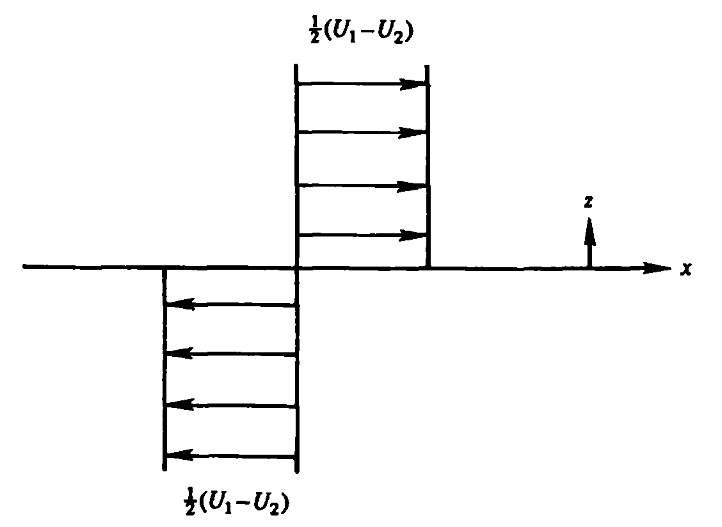
\includegraphics[width=0.9\textheight]{khpro.png}\\
  \caption{Velocity profile of a Kelvin-Helmholtz mode}\label{khpro}
\end{figure}

Kelvin-Helmholtz modes of instability is well found in the nature.
Figure \ref{khphoto} shows a billow cloud with the shape of
Kelvin-Helmholtz mode of waves.
\begin{figure}[htpb]
  \centering
  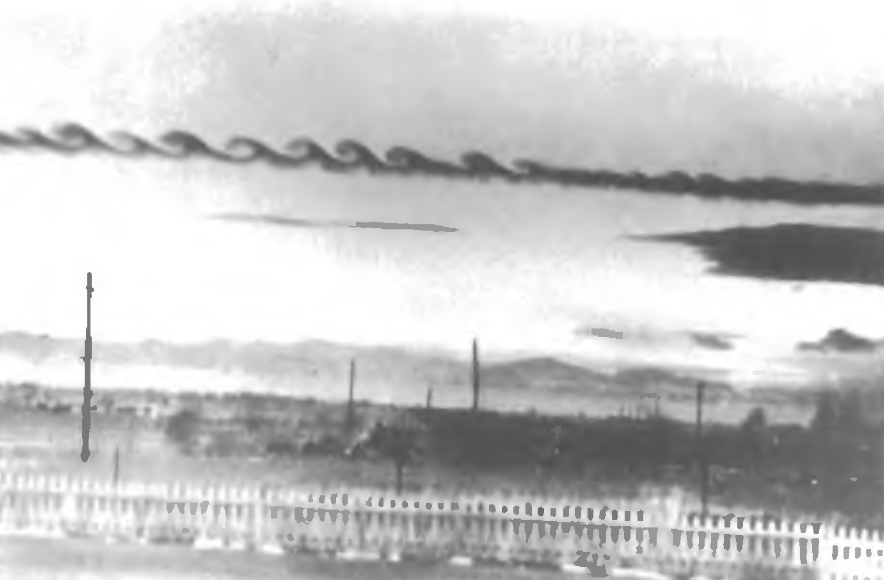
\includegraphics[width=0.9\textwidth]{khphoto.png}\\
  \caption{Billow cloud near Denver, Colorado (from \emph{Hydrodynamic Stability} by Drazin and Weid, \cite{Drazin})}\label{khphoto}
\end{figure}

\newslide
\subsection{Constant Density Flow}
For the velocity profile shown as below\footnote{Here I used the
transformation of reference frame to make $U_0=(U_1-U_2)/2$ in
\eqref{kh:pro} without the loss of generality.}
\begin{equation}\label{kh:bg}
\mathbf{U}(z) =
\begin{cases} U_0 \mathbf{i} &\text{if $z>0$,}\\
-U_0 \mathbf{i} &\text{if $z<0$.}
\end{cases}
\end{equation}
with $\rho=\rho_0$ everywhere and the boundary conditions $\phi \to
0$ as $z \to \pm\infty$, the solution of the Reyleigh's Stability
equation \eqref{kh:ray2} is in the form
\begin{equation*}
\phi =
\begin{cases}
Ae^{-\alpha z} &\text{if $z>0$,}\\
Be^{\alpha z} &\text{if $z<0$.}
\end{cases}
\end{equation*}
\newslide
There are two more boundary conditions at $z=0$:
\begin{enumerate}
  \item[(i)] The pressure at the interface must be continuous. From \eqref{kh:3-1}
  \begin{equation}
  \frac{\hat{p}}{\rho_0}=\frac{dU}{dz}\phi-(U-c)\frac{d\phi}{dz}\quad\text{is continuous.}\label{kh:b1}
  \end{equation}
  \item[(ii)] The displacement of the perturbed interface must be continuous. Let $z=z_0+\xi(x,t)$ be
  the displacement of the interface. The movement of the interface is given
  by
  \begin{align*}
  w'&=\frac{D\xi}{Dt}=\frac{\partial\xi}{\partial
  t}+(\mathbf{u}\cdot\nabla)\xi,\qquad
  \text{where }\mathbf{u}=\mathbf{U}(z)+\mathbf{u}'
  \end{align*}
  \newslide
Apply the linearization to drop the product of perturbed terms,
  let $\xi(x,t)=\hat{\xi}e^{i\alpha(x-ct)}$
  \begin{align}
  w'&=\frac{\partial\xi}{\partial t}+U\frac{\partial\xi}{\partial
  x}=-i\alpha c\,\xi+i\alpha U\xi\notag\\
  \hat{w}&=i\alpha(U-c)\hat{\xi}\notag\\
  -\hat{\phi}&=(U-c)\hat{\xi}\notag\\
  \frac{\phi}{U-c}&=-\hat{\xi}\quad\text{is continuous at $z=0$.}\label{kh:b2}
  \end{align}
\end{enumerate}
\newslide
Apply the boundary conditions from \eqref{kh:b1} and \eqref{kh:b2},
I get
\begin{subequations}\label{kh:lin}
\begin{align}
    (U_0-c)(-\alpha)A&=(-U_0-c)(\alpha)B\label{kh:lin1}\\
    \frac{A}{U_0-c}&=\frac{B}{-U_0-c}\label{kh:lin2}
\end{align}
\end{subequations}
Solving \eqref{kh:lin}, The solution is
\begin{equation}\label{lh:c}
    \boxed{c=\pm i U_0}
\end{equation}
\newslide
The result is plotted in Figure \ref{kh1}. There is one unstable
mode and one decaying mode corresponding to positive and negative
value of $c_I$ respectively. In Kelvin-Helmholtz instability, every
wave number $\alpha$ has a corresponding unstable mode.
\begin{figure}[htpb]
  \centering
  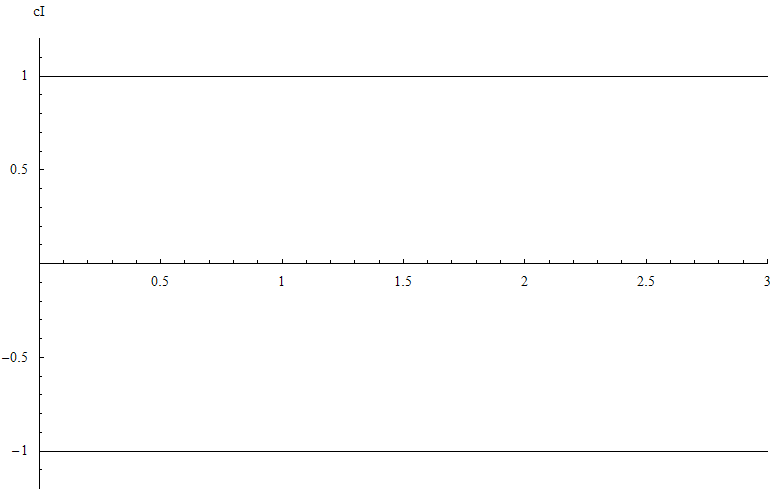
\includegraphics[width=0.9\textheight]{kh1.png}\\
  \caption{$c_I$ vs.~$\alpha$ for $U_0=1$ of a KH mode}\label{kh1}
\end{figure}

\newslide
\subsection{Density Stratified Flow}
For a velocity profile the same as in \eqref{kh:bg}
\begin{equation*}
\mathbf{U}(z) =
\begin{cases} U_0 \mathbf{i} &\text{if $z>0$,}\\
-U_0 \mathbf{i} &\text{if $z<0$.}
\end{cases}
\end{equation*}
with the boundary conditions $\phi \to 0$ as $z \to \pm\infty$,
$c=c_R+ic_I$ is complex in general. But the density is stratified by
a constant $N^2\equiv-(g/\rho_0)(d\rho/dz)$. The Boussinesq
approximation is applied so that the variation in density only
appears in the buoyancy term.
\newslide
Taylor-Goldstein equation \eqref{tay:eq2} is required to solve this
problem. By matching the boundary conditions at $z=0$ in general
case of \eqref{kh:pro}, I found $c_R=(U_1+U_2)/2$, which is
\begin{equation}\label{str:cr}
    c_R=\frac{U_0-U_0}{2}=0
\end{equation}
We have two types of solutions.
\newslide
\begin{enumerate}
\item[(A)] Neutral Solutions: $c_I=0$

For $\alpha^2>N^2/U^2$, the trial solution is
\begin{equation}\label{str:tr1}
\phi =
\begin{cases}
Ae^{-nz} &\text{if $z>0$,}\\
Be^{nz} &\text{if $z<0$.}
\end{cases}
\qquad \text{where }n=\sqrt{\alpha^2-\frac{N^2}{U^2}}
\end{equation}
Matching boundary conditions at $z=0$:
\begin{enumerate}
  \item[(i)] pressure: $-nU_0A=n(-U_0)B \quad\Rightarrow A=B$
  \item[(ii)] displacement: $A/U_0=B/{-U_0} \quad\Rightarrow A={-B}$
\end{enumerate}
Therefore $A=B=0$. There is no neutral solution for
$\alpha^2>N^2/U^2$.
\newslide
For $\alpha^2<N^2/U^2$, the trial solution is
\begin{equation}\label{str:tr2}
\phi =
\begin{cases}
Ae^{inz} &\text{if $z>0$,}\\
Be^{inz} &\text{if $z<0$.}
\end{cases}
\qquad \text{where }n=\pm\sqrt{\frac{N^2}{U^2}-\alpha^2}
\end{equation}
Matching boundary conditions at $z=0$:
\begin{enumerate}
  \item[(i)] pressure: $-inU_0A=-in(-U_0)B \quad\Rightarrow A={-B}$
  \item[(ii)] displacement: $A/U_0=B/{-U_0} \quad\Rightarrow A={-B}$
\end{enumerate}
\newslide
To satisfy the radiative boundary conditions at $z \to \pm\infty$,
we have the vertical components of the energy flux
as\footnote{$\langle\quad\rangle$ means average value.}
\begin{align}
    \langle F_z\rangle&=\langle\text{Re}(p')\text{Re}(w')\rangle\notag\\
    &=\langle\text{Re}(-inU\phi e^{i(\alpha x-\alpha c t)})\text{Re}(-i\alpha\phi e^{i(\alpha x-\alpha c t)})\rangle\notag\\
    &=\frac{1}{2}\text{Re}(nU\alpha\phi^*e^{-i(\alpha x-\alpha c t)}\phi e^{i(\alpha x-\alpha c t)})\notag\\
    &=\frac{1}{2}\text{Re}(nU\alpha\phi^*\phi)\notag\\
    &=\frac{1}{2}nU\alpha\lvert A\rvert^2\label{str:rad}
\end{align}
\newslide
For $z>0$,
\begin{equation*}
    U=U_0,\quad\langle F_z\rangle>0 \quad\Rightarrow n>0
\end{equation*}
For $z<0$,
\begin{equation*}
    U=-U_0,\quad\langle F_z\rangle<0 \quad\Rightarrow n>0
\end{equation*}
\newslide
Therefore the natural solution is
\begin{equation}\label{str:sol1}
\phi =
\begin{cases}
Ae^{inz} &\text{if $z>0$,}\\
-Ae^{inz} &\text{if $z<0$.}
\end{cases}
\qquad \text{where }n=\sqrt{\frac{N^2}{{U_0}^2}-\alpha^2},\quad
\alpha^2<\frac{N^2}{{U_0}^2}
\end{equation}
\begin{equation}\label{str:c1}
    \boxed{c=0,\qquad\alpha^2<\frac{N^2}{{U_0}^2}}
\end{equation}
\newslide
\item[(B)] Unstable Solutions: $c_I\neq0$

The trial solution is
\begin{equation}\label{str:tr3}
\phi =
\begin{cases}
Ae^{-nz} &\text{if $z>0$,}\\
Be^{n^*z} &\text{if $z<0$.}
\end{cases}
\qquad \text{where }n^2=\alpha^2-\frac{N^2}{(U-ic_I)^2}
\end{equation}
$n$ is chosen to have positive real part so that the solution
vanishes when $z \to \pm\infty$. When $\text{Re}(n)=0$,
$\text{Im}(n)<0$ which automatically satisfied the radiative
boundary conditions as shown in \eqref{str:rad}.
\newslide
Matching boundary conditions at $z=0$:
\begin{enumerate}
  \item[(i)] pressure: $n(U_0-ic_I)A=n^*(U_0+ic_I)B$
  \item[(ii)] displacement: $A/(U_0-ic_I)=B/({-U_0}-ic_I)$
\end{enumerate}
Combining the two equations to get
\begin{equation}\label{str:b1}
    n(U_0-ic_I)^2=-n^*(U_0+ic_I)^2
\end{equation}
Which can be written as $n(U_0-ic_I)^2 = -(n(U_0-ic_I)^2)^*$,
therefore I have
\begin{equation}
    \text{Re}\Bigl(n(U_0-ic_I)^2\Bigr)=0\label{str:b2}
\end{equation}
\newslide
Then expand $n(U_0-ic_I)^2$ as
\begin{equation}
    n(U_0-ic_I)^2=({U_0}^2-2iU_0c_I-{c_I}^2)(n_R+in_I)\label{str:b3}
\end{equation}
By comparing real part of \eqref{str:b2} and \eqref{str:b3},
\begin{equation}
    n_R=-\frac{2c_IU_0}{{U_0}^2-{c_I}^2}n_I\label{str:b4}
\end{equation}
\newslide
Write $n$ as
$n=n_R+in_I=\Bigl(-\frac{2c_IU_0}{{U_0}^2-{c_I}^2}+1\Bigr)n_I$, take
square and compare the real and imaginary parts with the definition
in \eqref{str:tr3}, I get
\begin{align}
    {c_I}^2 &={U_0}^2-\frac{N^2}{2\alpha^2},\qquad\text{where }\alpha^2>\frac{N^2}{2{U_0}^2}\label{str:sol1}\\
    n^2 &=-\alpha^2\frac{(U+ic_I)^2}{(U-ic_I)^2}\label{str:sol2}
\end{align}
\newslide
$c$ is found to be:
\begin{equation}\label{str:c2}
    \boxed{c=\pm
    i\sqrt{{U_0}^2-\frac{N^2}{2\alpha^2}},\qquad\alpha^2>\frac{N^2}{2{U_0}^2}}
\end{equation}
\end{enumerate}
The unstable solution is plotted in Figure \ref{kh2}. The density
stratification tends to stabilize long waves with smaller wave
number $\alpha$.
\begin{figure}[htpb]
  \centering
  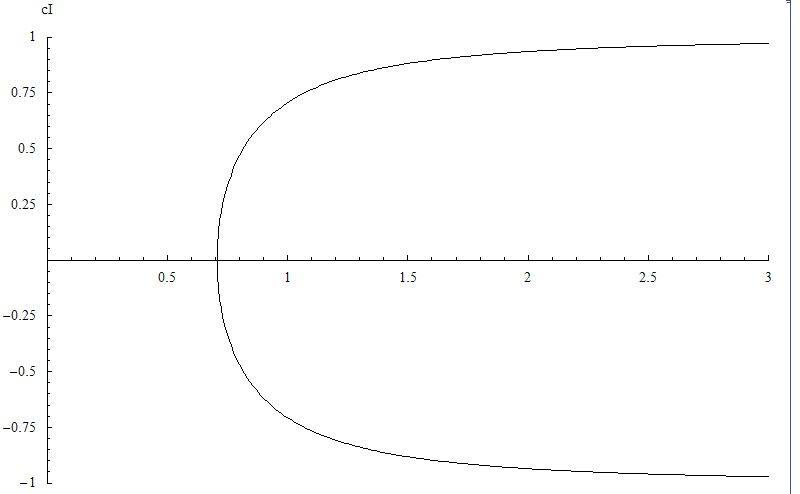
\includegraphics[width=0.9\textheight]{kh2.png}\\
  \caption{$c_I$ vs.~$\alpha$ for $U_0=1$ of a stratified KH mode}\label{kh2}
\end{figure}

%-----------------------------------------------------------
\newslide
\section{Holmboe Instability} Holmboe instability is defined by the
velocity profile:
\begin{equation}\label{ho:pro}
\mathbf{U}(z) =
\begin{cases}
U_0 \mathbf{i} &\text{if $z>d$,}\\
\dfrac{z}{d}U_0\mathbf{i} &\text{if $-d<z<d$,}\\
-U_0 \mathbf{i} &\text{if $z<-d$.}
\end{cases}
\end{equation}
Or, in dimensionless form:
\begin{equation}\label{ho:pro2}
\mathbf{U}(z) =
\begin{cases}
1 \mathbf{i} &\text{if $z>1$,}\\
\dfrac{z}{d}U_0\mathbf{i} &\text{if $-1<z<1$,}\\
-1 \mathbf{i} &\text{if $z<-1$.}
\end{cases}
\end{equation}

The velocity profile is shown in Figure \ref{hopro}.
\begin{figure}[htpb]
  \centering
  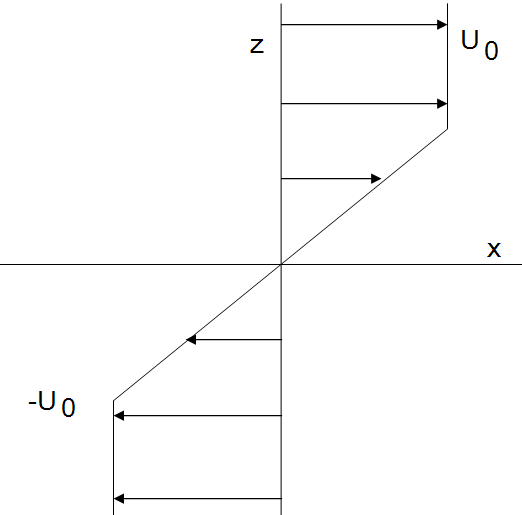
\includegraphics[width=0.9\textheight]{hopro.png}\\
  \caption{Velocity profile of a Holmboe mode}\label{hopro}
\end{figure}

\newslide
\section{Constant Density Flow}
For the profile in \eqref{ho:pro2} with constant density
$\rho=\rho_0$ everywhere, the trial solution of the Reyleigh's
Stability equation \eqref{kh:ray2} is in the form
\begin{equation}\label{hom:con0}
\phi =
\begin{cases}
Ae^{-\alpha z} &\text{if $z>1$,}\\
Be^{-\alpha z} + Ce^{\alpha z} &\text{if $-1<z<1$,}\\
De^{\alpha z} &\text{if $z<-1$.}
\end{cases}
\end{equation}

At $z=1$, the boundary conditions are:
\begin{enumerate}
  \item[(i)] pressure:
  \begin{align}
    \hat{p}&=U'\phi-(U-c)\phi'\quad \text{is continuous}\notag\\
    -(1-c)Ae^{-\alpha}&=Be^{-\alpha} + Ce^{\alpha}-(1-c)\alpha(-B
    e^{-\alpha}+Ce^{\alpha})\label{hom:con1}
  \end{align}
  \item[(ii)] displacement:
  \begin{align}
    \phi &\quad \text{is continuous}\notag\\
    Ae^{-\alpha}&=Be^{-\alpha} + Ce^{\alpha}\label{hom:con2}
  \end{align}
\end{enumerate}
Substitute \eqref{hom:con2} into \eqref{hom:con1}, I get
\begin{equation}\label{hom:con3}
    2(1-c)\alpha C=Be^{-2\alpha}+C
\end{equation}

At $z=-1$, the boundary conditions are:
\begin{enumerate}
  \item[(i)] pressure:
  \begin{equation}
    -(-1-c)Ae^{\alpha}=Be^{\alpha} + Ce^{-\alpha}-(-1-c)\alpha(-B
    e^{\alpha}+Ce^{-\alpha})\label{hom:con4}
  \end{equation}
  \item[(ii)] displacement:
  \begin{equation}
    Be^{\alpha} + Ce^{-\alpha}=De^{\alpha}\label{hom:con5}
  \end{equation}
\end{enumerate}
Substitute \eqref{hom:con5} into \eqref{hom:con4}, I get
\begin{equation}\label{hom:con6}
    2(1+c)\alpha B=B+Ce^{-2\alpha}
\end{equation}

Combining \eqref{hom:con3} and \eqref{hom:con6} to eliminate the
constants $B$ and $C$, I found that the non-dimensional phrase speed
satisfy the equation:
\begin{equation}\label{hom:con}
    \boxed{c^2+\Bigl(\frac{e^{-4\alpha}-(2\alpha-1)^2}{4\alpha^2}\Bigr)=0}
\end{equation}
The solution is
\begin{equation}\label{hom:con7}
    c=\pm\sqrt{\Bigl(1-\frac{1}{2\alpha}\Bigr)^2-\Bigl(\frac{1}{4\alpha^2}\Bigr)e^{-4\alpha}}
\end{equation}

The value of $\alpha$ was solved numerically. For $\alpha>0.639232$,
$c$ is real, the solution is neutral. For $0\leq\alpha\leq0.639232$,
$c$ is imaginary, one of the solutions is unstable. The value of
$c_R$ and $c_I$ is plotted in Figure \ref{ho1} and \ref{ho2}. From
the graph we can verify that when $\alpha \rightarrow 0$, $c=\pm i$,
this recovers the result of Kelvin-Helmholtz instability.
\begin{figure}[htpb]
  \centering
  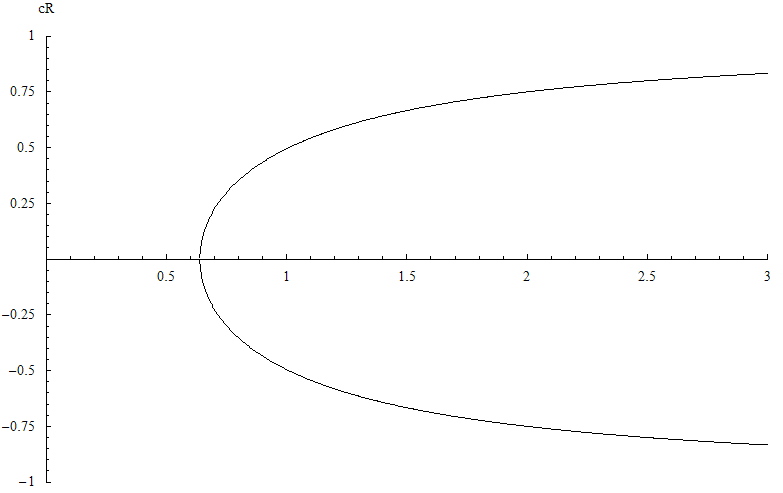
\includegraphics[width=0.9\textwidth]{ho1.png}\\
  \caption{$c_R$ vs.~$\alpha$ for $U_0=1$ of a Holmboe mode}\label{ho1}
\end{figure}
\begin{figure}[htpb]
  \centering
  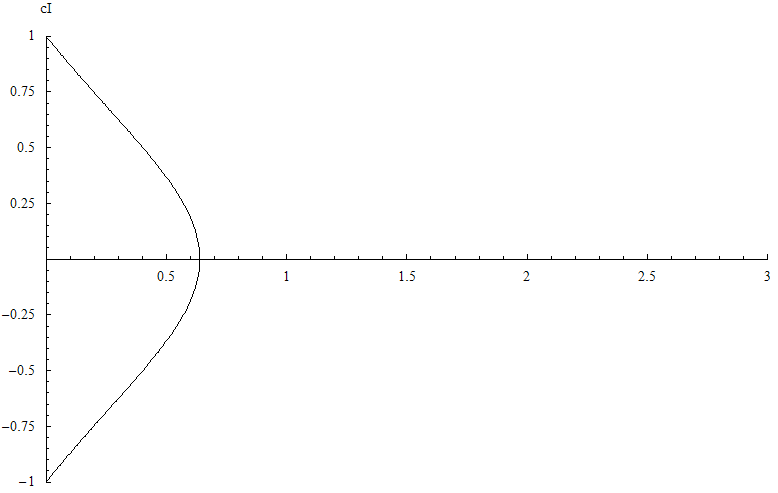
\includegraphics[width=0.9\textwidth]{ho2.png}\\
  \caption{$c_I$ vs.~$\alpha$ for $U_0=1$ of a Holmboe mode}\label{ho2}
\end{figure}

\newslide
\section{Sheared Density Flow}
Consider the same velocity profile as  \eqref{ho:pro2} but with a
sheared density profile:
\begin{equation}\label{she1}
\rho =
\begin{cases}
\rho_0 &\text{if $z>0$,}\\
\rho_0+\Delta\rho &\text{if $z<0$,}\\
\end{cases}
\end{equation}
The trial solution is
\begin{equation}\label{she2}
\phi =
\begin{cases}
Ae^{-\alpha z} &\text{if $z>1$,}\\
Be^{-\alpha z} + Ce^{\alpha z} &\text{if $0<z<1$,}\\
De^{-\alpha z} + Ee^{\alpha z} &\text{if $-1<z<0$,}\\
Fe^{\alpha z} &\text{if $z<-1$.}
\end{cases}
\end{equation}
Using the same technique as last section, we get at $z=1$
\begin{equation}\label{she3}
    2(1-c)\alpha C=Be^{-2\alpha}+C
\end{equation}
and at $z=-1$
\begin{equation}\label{she4}
    2(1+c)\alpha D=D+Ee^{-2\alpha}
\end{equation}
However, the fluid near $z=0$ is affected by the buoyancy force due
to the density shearing, so I have to treat it with a different
method. First, by matching $\phi$, I get
\begin{equation}\label{she5}
    B+C=D+E
\end{equation}
Using the vorticity equation cited in Caulfield
\cite{Caulfield}\footnote{The result is following Hoiland, 1948.},
the $x$ component can be written as
\begin{equation}\label{she6}
    \frac{D}{Dt}\Bigl(\frac{\partial u}{\partial z}\Bigr)=
    \Bigl(g'\frac{\partial \xi}{\partial x}\Bigr)\delta(z-\xi)
\end{equation}
where $u=U(z)+u'$ is the total velocity in $x$ direction,
$g'=g\Delta\rho/\rho$ is the reduced gravitational acceleration,
$\xi$ is the perturbed displacement of the interface with density
jump $\Delta\rho$. Note that $U(0)=0$ at $z=0$ and linearizing, I
found that $u=u'$ and $D/Dt=\partial/\partial t$ at $z=0$. Integrate
\eqref{she6} over an arbitrary small region near the density
interface, I obtain
\begin{equation}\label{she7}
    \frac{\partial}{\partial t}(u'_+-u'_-)= g'\frac{\partial \xi}{\partial
    x}\quad \text{at $z=0$.}
\end{equation}
From \eqref{kh:b2},
\begin{equation}\label{she8}
\hat{\xi}=-\frac{\phi}{U-c}=\frac{\phi}{c}\quad\text{at $z=0$.}
\end{equation}
Recall that $u'=(d\phi/dz) e^{i\alpha( x - ct)}$ and $\xi=\hat\xi
e^{i\alpha( x - ct)}$, I can write \eqref{she7} in
\begin{align*}
    \frac{\partial}{\partial t}\Bigl[\frac{d(\phi_+-\phi_-)}{dz}e^{i\alpha( x - ct)}\Bigr]
    &= g'\frac{\partial}{\partial
    x}(\hat\xi e^{i\alpha( x - ct)})\\
    -i\alpha c[\alpha(-B+C+D-E)\phi e^{i\alpha( x - ct)}]
    &= g'(i\alpha\hat\xi e^{i\alpha( x - ct)})\\
    c\alpha(B-C-D+E)\phi &= g'\frac{\phi}{c}
\end{align*}
Define the bulk Richardson number as
\begin{equation}\label{she10}
    Ri_0=\frac{g\Delta\rho d}{\rho(\Delta u)^2}=\frac{g' 2}{2^2}=\frac{g'}{2}
\end{equation}
where $d$ is the thickness of the shear layer and $\Delta u$ is the
velocity difference of the upper and lower region. Finally I get
\begin{equation}\label{she11}
    B-C=D-E+\frac{2Ri_0}{\alpha c^2}
\end{equation}
Put together \eqref{she3}, \eqref{she4}, \eqref{she5} and
\eqref{she11}, we get the stability equation for a sheared density
flow:
\begin{equation}\label{she12}
\boxed{c^4+\Bigl(\frac{e^{-4\alpha}-(2\alpha-1)^2}{4\alpha^2}-\frac{Ri_0}{\alpha}\Bigr)c^2
+\frac{Ri_0}{\alpha}\Bigl(\frac{e^{-2\alpha}+(2\alpha-1)}{2\alpha}\Bigr)^2=0}
\end{equation}

The result is visualized by Lawrence et al.~\cite{Lawrence} in
Figure \ref{ho3}. The region I shows Kelvin-Helmholtz instability
while region II shows Holmboe instability.
\begin{figure}[htpb]
  \centering
  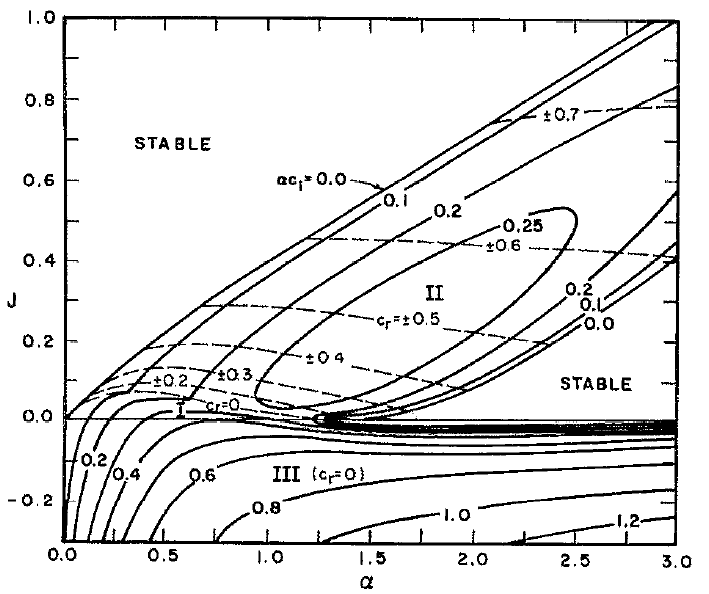
\includegraphics[width=0.9\textwidth]{ho3.png}\\
  \caption{Stability diagram for different $Ri_0$ and $\alpha$}\label{ho3}
\end{figure}

%-----------------------------------------------------------
\newslide
\chapter{Discussion}
The simple problems of Kelvin-Helmholtz instability and Holmboe
instability were investigated in this project. However, only limited
results can be done analytically. For some more complicated
problems, such as non-zero depth density shear layer, mixing of
fluids, need to be done computationally. For example, Smyth and
Winters \cite{Smyth} have done some computations on the three
dimensional time evolution of Kelvin-Helmholtz and Holmboe modes of
waves. The results are shown in Figure \ref{kh3} and Figure
\ref{ho5}. Note that there are transition from Kelvin-Helmholtz to
Holmboe mode in Figure \ref{kh3}(c).
\begin{figure}[htpb]
  \centering
  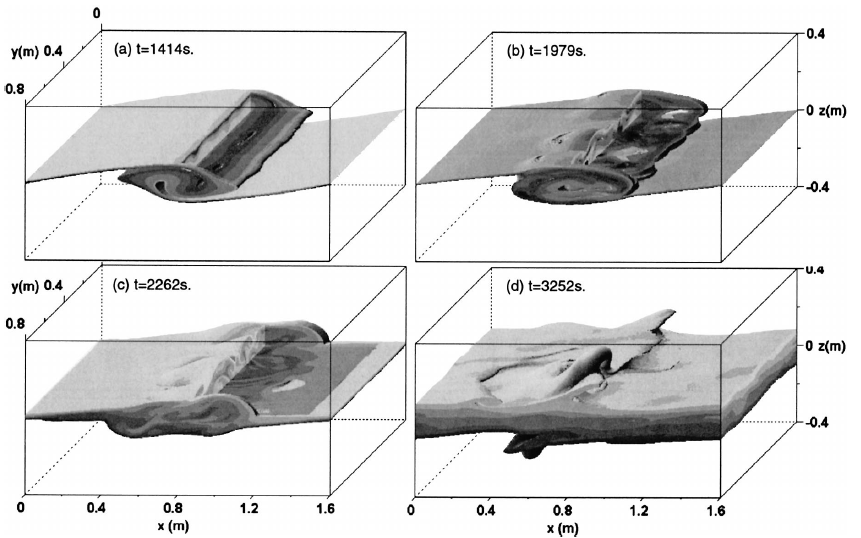
\includegraphics[width=0.9\textwidth]{kh3.png}\\
  \caption{Time evolution for a Kelvin-Helmholtz mode (Smyth and Winters \cite{Smyth})}\label{kh3}
\end{figure}
\begin{figure}[htpb]
  \centering
  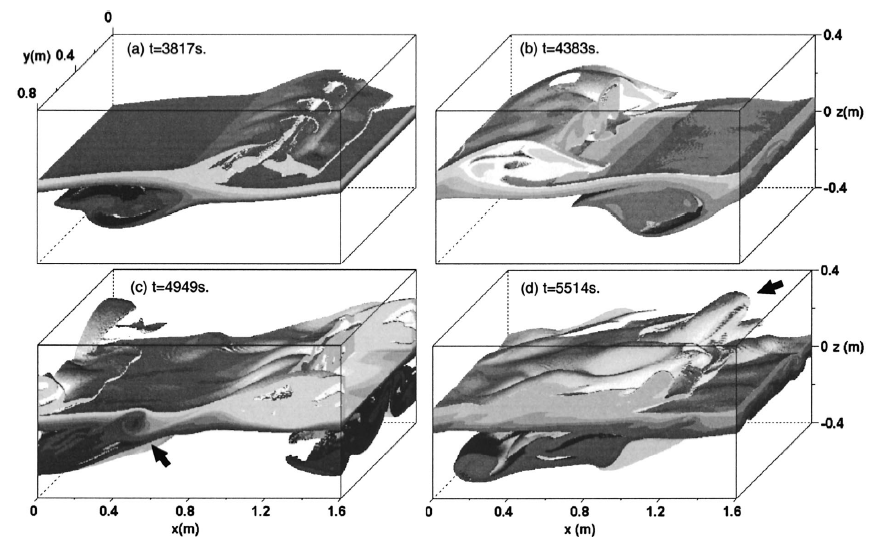
\includegraphics[width=0.9\textwidth]{ho5.png}\\
  \caption{Time evolution for a Holmboe mode (Smyth and Winters \cite{Smyth})}\label{ho5}
\end{figure}

%-----------------------------------------------------------
\newslide
\section*{Acknowledgements}
\addcontentsline{toc}{section}{\numberline{}Acknowledgements} Thanks
to the University of Toronto and The Chinese University of Hong Kong
for offering me the opportunity to attend this exchange program in
the University of Toronto. Thanks to the Department of Physics in
the University of Toronto for offering me this undergraduate
research project. Thanks to Prof.~W.R.~Peltier for being my
supervisor in this project.

\newslide
\begin{thebibliography}{99}
\addcontentsline{toc}{section}{\numberline{}Bibliography}
\bibitem{Batchelor} G.K.~Batchelor, 1967, \emph{Introduction to Fluid Mechanics},
Chapter 1--3
\bibitem{Caulfield} C.P.~Caulfield, 1994, \emph{Multiple Linear
Instability of Layered Stratified Shear Flow}, J.~Fluid
Mech.~vol.~258 pp.~255--285
\bibitem{Drazin} P.G.~Drazin and W.H.~Reid, 1981, \emph{Hydrodynamic Stability},
Chapter 4
\bibitem{Drazin2} P.G.~Drazin, 2002, \emph{Introduction to Hydrodynamic
Stability}, Chapter 8
\bibitem{Lawrence} G.A.~Lawrence et al., 1991, \emph{The Stability of a Sheared Density Interface},
Phys.~Fluids A 3 (10) 2360
\newpage
\bibitem{Tensor} H.~Jeffreys, 1961, \emph{Cartesian Tensors}, Chapter VII
\bibitem{Kundu} P.K.~Kundu and I.M.~Cohen, 2002, \emph{Fluid Mechanics}, Chapter
4 and 12
\bibitem{460S} W.R.~Peltier, \emph{PHY460S Lecture Notes}, Chapter 1
\bibitem{Smyth} W.D.~Smyth and K.B.~Winters, 2002, \emph{Turbulence and Mixing in Holmboe
Waves}, Journal of Physical Oceanography Vol.33 694
\end{thebibliography}

%\appendix
%\chapter{Mathematical Proofs}
%\section{Torque on a Fluid Packet}
%\section{Isotropic Tensors}
%-----------------------------------------------------------
\end{slide}
\end{document}
